% ****** Start of file apssamp.tex ******
%
%   This file is part of the APS files in the REVTeX 4.2 distribution.
%   Version 4.2a of REVTeX, December 2014
%
%   Copyright (c) 2014 The American Physical Society.
%
%   See the REVTeX 4 README file for restrictions and more information.
%
% TeX'ing this file requires that you have AMS-LaTeX 2.0 installed
% as well as the rest of the prerequisites for REVTeX 4.2
%
% See the REVTeX 4 README file
% It also requires running BibTeX. The commands are as follows:
%
%  1)  latex apssamp.tex
%  2)  bibtex apssamp
%  3)  latex apssamp.tex
%  4)  latex apssamp.tex
%
\documentclass[%
 reprint,
%superscriptaddress,
%groupedaddress,
%unsortedaddress,
%runinaddress,
%frontmatterverbose, 
%preprint,
%preprintnumbers,
%nofootinbib,
%nobibnotes,
%bibnotes,
 amsmath,amssymb,
 aps,
%pra,
%prb,
%rmp,
%prstab,
%prstper,
%floatfix,
onecolumn
]{revtex4-2}

\usepackage{graphicx}% Include figure files
\usepackage{dcolumn}% Align table columns on decimal point
\usepackage{bm}% bold math
% \usepackage{extarrows} % write text up the arrows.
\usepackage{hyperref}% add hypertext capabilities
%\usepackage[mathlines]{lineno}% Enable numbering of text and display math
%\linenumbers\relax % Commence numbering lines

%\usepackage[showframe,%Uncomment any one of the following lines to test 
%%scale=0.7, marginratio={1:1, 2:3}, ignoreall,% default settings
%%text={7in,10in},centering,
%%margin=1.5in,
%%total={6.5in,8.75in}, top=1.2in, left=0.9in, includefoot,
%%height=10in,a5paper,hmargin={3cm,0.8in},
%]{geometry}

\hypersetup{colorlinks=true,
            linkcolor=blue,
            anchorcolor=blue,
            citecolor=blue}



            
\begin{document}

\preprint{APS/123-QED}
\allowdisplaybreaks[1]

\title{Calculation of three modes interferometer with displacement 
operators}

\author{zz}
%  \altaffiliation[Also at ]{Physics Department, XYZ University.}%Lines break automatically or can be forced with \\

% \affiliation{%
%  Authors' institution and/or address
% }%

% \date{\today}
\date{February 1, 2021}

\begin{abstract}
In this manuscript I try to describe the whole physical system of 
three modes interferometer with displacement operators. I successfully
finish the calculation that input state $ \left |1,1,1 \right \rangle $
passes the tritter(three ports beam-splitters). And I also try to apply
displament operators to the following states. I didn't know how to 
slove it at first, but later on I found a solution to the problem and
probably solved the problem correctly.
\end{abstract}

%\keywords{Suggested keywords}%Use showkeys class option if keyword  %display desired
\maketitle






\subsection{Analyzation of tritter with the input state $\left|1,1,1\right\rangle$}

\begin{figure}[h]
  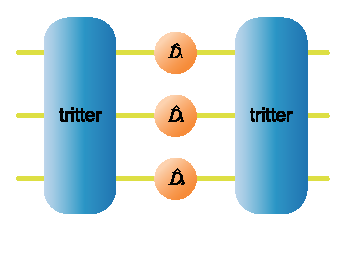
\includegraphics{image/triMZI.eps}
  \caption{\label{fig:triMZI} Three modes interferometer with tritter
  (three ports beam splitters) and displacement transformation.}
\end{figure}

% unitary operator
Like many articles do, the unitary transformation of the tritter
(three ports beam-splitters) has the following form:
\begin{equation}
  \hat{U} = \frac{1}{\sqrt{3}}
  \begin{pmatrix}
  1 & e^{i\frac{2\pi}{3}} & e^{i\frac{2\pi}{3}} \\
  e^{i\frac{2\pi}{3}} & 1 & e^{i\frac{2\pi}{3}} \\
  e^{i\frac{2\pi}{3}} & e^{i\frac{2\pi}{3}} & 1 
  \end{pmatrix}
  % ab12345678abc123456abcdef\alpha\beta\gamma\delta1234556\alpha\beta
  % \frac{1\sum^{a}_{b}}{A^2}%
  ~.
\end{equation}

This unitary operator and creation operator have the following 
connection:
\begin {equation}
\hat{b_i}^\dagger = 
\begin{matrix} \sum_{i,j} U_{ij}\hat{a_j}^\dagger \end{matrix}~,
\end{equation}

where the $\hat{a}^\dagger$ and $\hat{b}^\dagger$ are creation 
operator of the input and output modes respectively.

Or we can rewrite it in matrix form:
\begin {equation}
\overrightarrow{\hat{b}^\dagger} = 
\hat{U}\overrightarrow{\hat{a}^\dagger}
,~and~~
\overrightarrow{\hat{a}^\dagger} = 
\hat{U}^{-1}\overrightarrow{\hat{b}^\dagger}
=\hat{U}^\dagger\overrightarrow{\hat{b}^\dagger}
~.
\end{equation}

For the input state $\left|1,1,1\right\rangle$, we have:
\begin{equation}
\left|1,1,1\right\rangle = \hat{a}_1^\dagger\hat{a}_2^\dagger
\hat{a}_3^\dagger \left|0,0,0\right\rangle.
\end{equation}

Because tritter doesn't change the number of photon, so the state
$\left|0,0,0\right\rangle$ has a special character:
\begin{equation}
  \left|0,0,0\right\rangle_{in} ~\xrightarrow{Tritter}~
  \left|0,0,0\right\rangle_{out}.
\end{equation}

% calculation of 111.
Therefore, for the input state $\left|1,1,1\right\rangle$,
changing the creation operators, note that the conjugate of 
$\hat{U}$ should be taken here:
\begin{eqnarray}
  \hat{a}_1^\dagger\hat{a}_2^\dagger\hat{a}_3^\dagger 
  \left|0,0,0\right\rangle_{in} 
  ~\xrightarrow{Tritter}~&&
  \frac{1}{3\sqrt{3}}
  \left(
    \hat{b}_1^\dagger + e^{-i\frac{2\pi}{3}}\hat{b}_2^\dagger +
    e^{-i\frac{2\pi}{3}}\hat{b}_3^\dagger
  \right)
  \left(
    e^{-i\frac{2\pi}{3}}\hat{b}_1^\dagger + \hat{b}_2^\dagger +
    e^{-i\frac{2\pi}{3}}\hat{b}_3^\dagger
  \right)
  \left(
    e^{-i\frac{2\pi}{3}}\hat{b}_1^\dagger + 
    e^{-i\frac{2\pi}{3}}\hat{b}_2^\dagger + \hat{b}_3^\dagger
  \right)
  \left|0,0,0\right\rangle_{out}. \nonumber \\
  =&&\frac{1}{3\sqrt{3}}
  \biggl[
    e^{i\frac{2\pi}{3}}\hat{b}_1^{\dagger 3} + 
    e^{i\frac{2\pi}{3}}\hat{b}_2^{\dagger 3} +
    e^{i\frac{2\pi}{3}}\hat{b}_3^{\dagger 3} +
    \left(1+e^{i\frac{2\pi}{3}}+e^{-i\frac{2\pi}{3}}\right)
    \hat{b}_1^{\dagger 2} \hat{b}_2^{\dagger} +
    \left(1+e^{i\frac{2\pi}{3}}+e^{-i\frac{2\pi}{3}}\right)
    \hat{b}_1^{\dagger 2} \hat{b}_3^{\dagger} \nonumber \\ &&+
    \left(1+e^{i\frac{2\pi}{3}}+e^{-i\frac{2\pi}{3}}\right)
    \hat{b}_1^{\dagger} \hat{b}_2^{\dagger 2} +
    \left(1+e^{i\frac{2\pi}{3}}+e^{-i\frac{2\pi}{3}}\right)
    \hat{b}_1^{\dagger} \hat{b}_3^{\dagger 2} +
    \left(1+e^{i\frac{2\pi}{3}}+e^{-i\frac{2\pi}{3}}\right)
    \hat{b}_2^{\dagger 2} \hat{b}_3^{\dagger} \nonumber \\ &&+
    \left(1+e^{i\frac{2\pi}{3}}+e^{-i\frac{2\pi}{3}}\right)
    \hat{b}_2^{\dagger} \hat{b}_3^{\dagger 2}
  \biggr]
  \left|0,0,0\right\rangle_{out} \nonumber  \\
  =&& \frac{1}{3\sqrt{3}}
  \left[
    e^{i\frac{2\pi}{3}}\hat{b}_1^{\dagger 3} + 
    e^{i\frac{2\pi}{3}}\hat{b}_2^{\dagger 3} +
    e^{i\frac{2\pi}{3}}\hat{b}_3^{\dagger 3} +
    3\left(1+e^{i\frac{2\pi}{3}}\right)\hat{b}_1^\dagger
    \hat{b}_2^\dagger\hat{b}_3^\dagger
  \right]
  \left|0,0,0\right\rangle_{out} \nonumber \\
  =&&
  \left[
    \left(-\frac{1}{6\sqrt{3}}+\frac{i}{6}\right)
    \left( \hat{b}_1^{\dagger 3} + \hat{b}_2^{\dagger 3} +
    \hat{b}_3^{\dagger 3} \right) +
    \left(\frac{1}{2\sqrt{3}}+\frac{i}{2}\right)
    \hat{b}_1^\dagger\hat{b}_2^\dagger\hat{b}_3^\dagger
  \right]
  \left|0,0,0\right\rangle_{out} \nonumber \\
  =&& 
  \left(-\frac{\sqrt{2}}{6}+\frac{i}{\sqrt{6}}\right)
  \left(
    \left|3,0,0\right\rangle+\left|0,3,0\right\rangle+
    \left|0,0,3\right\rangle
  \right) +
  \left(\frac{1}{2\sqrt{3}}+\frac{i}{2}\right)
  \left|1,1,1\right\rangle.
\end{eqnarray}          


% Displacement operators
\subsection{Displacement for the following states}
After passing the tritter, photons are effected by the displacement operators
in three modes, $\hat{D}_1, \hat{D}_2 \text{and} \hat{D}_3$, respectively.
With the identity(the disentangling theorem):
\begin{equation}
  e^{\hat{A}+\hat{B}}=e^{\hat{A}}e^{\hat{B}}e^{-\frac{1}{2}\left[\hat{A},\hat{B}\right]} .
\end{equation}
when $\hat{A}=\alpha\hat{a}^\dagger$ and $\hat{B}=-\alpha^*\hat{a}$,
we can the rewrite displacement operator:
\begin{equation}
  \hat{D}(\alpha) = e^{(\alpha\hat{a}^\dagger-\alpha^*\hat{a})}
  = e^{-\frac{1}{2}|\alpha|^2}e^{\alpha\hat{a}^\dagger}e^{-\alpha^*\hat{a}} .
\end{equation}

% displacement for n00
Because of the superposition principle, we can consider the state 
$ \left|1,1,1\right\rangle \text{and} \left|3,0,0\right\rangle\dots $ separately.
\subsubsection{ $|n,0,0\rangle$ states}
Firstly, we consider a more general case,
the $\hat{D}_1(\alpha_1)$ operator act on $\left|n,0,0\right\rangle$:
\begin{eqnarray}
  \hat{D}_1(\alpha_1) \left|n,0,0\right\rangle =&&
  e^{-\frac{1}{2}|\alpha_1|^2}e^{\alpha_1\hat{a}_1^\dagger}e^{-\alpha_1^*\hat{a}_1}
  \left|n,0,0\right\rangle \nonumber \\
  =&& e^{-\frac{1}{2}|\alpha_1|^2}e^{\alpha_1\hat{a}_1^\dagger}
  \sum_{k=0}^{+\infty}\frac{{(-\alpha_1^*\hat{a}_1)}^k}{k!} 
  \left|n,0,0\right\rangle  \nonumber \\
  =&& e^{-\frac{1}{2}|\alpha_1|^2}e^{\alpha_1\hat{a}_1^\dagger}
  \sum_{k=0}^{n}\frac{{(-\alpha_1^*)}^k}{k!} \sqrt{\frac{n!}{(n-k)!}}
  |n-k,0,0\rangle \nonumber \\
  =&& e^{-\frac{1}{2}|\alpha_1|^2} 
  \sum_{l=0}^{+\infty}\frac{{(\alpha_1\hat{a}_1^\dagger)}^l}{l!}
  \sum_{k=0}^{n}\frac{{(-\alpha_1^*)}^k}{k!} \sqrt{\frac{n!}{(n-k)!}}
  |n-k,0,0\rangle 
  \nonumber \\
  =&& e^{-\frac{1}{2}|\alpha_1|^2} \sum_{k=0}^{n} \sum_{l=0}^{+\infty}
  \alpha_1^l {(-\alpha_1^*)}^k \frac{\sqrt{n!(n-k+l)!}}{k!~l!~(n-k)!}
  |n-k+l,0,0\rangle 
  \label{D1|n00}
\end{eqnarray}

So, for the $|3,0,0\rangle$ we have:
\begin{equation}
  \hat{D}_1(\alpha_1) |3,0,0\rangle =
  e^{-\frac{1}{2}|\alpha_1|^2} \sum_{k=0}^{3} \sum_{l=0}^{+\infty}
  \alpha_1^l {(-\alpha_1^*)}^k \frac{\sqrt{3!(3-k+l)!}}{k!~l!~(3-k)!}
  |3-k+l,0,0\rangle .
\end{equation}

other circumstances are similar to this.

% displacement for 111
\subsubsection{ $|1,1,1\rangle$ state}
We want to calculate the 
$ \hat{D}_1(\alpha_1)\hat{D}_2(\alpha_2)\hat{D}_3(\alpha_3) |1,1,1\rangle$.
Because $\hat{D}_1, \hat{D}_2 \text{~and~} \hat{D}_3$ is commute,
so which of them are calculated first doesn't matter.
Here we start from $\hat{D}_1(\alpha_1)$:
\begin{eqnarray}
  \hat{D}_1(\alpha_1) |1,1,1\rangle =&&
  e^{-\frac{1}{2}|\alpha_1|^2}e^{\alpha_1\hat{a}_1^\dagger}
  e^{-\alpha_1^*\hat{a}_1} |1,1,1\rangle 
  \nonumber \\ =&&
  e^{-\frac{1}{2}|\alpha_1|^2}e^{\alpha_1\hat{a}_1^\dagger}
  \sum_{k=0}^{+\infty}\frac{{(-\alpha_1^*\hat{a}_1)}^k}{k!}
  |1,1,1\rangle 
  \nonumber \\ =&&
  e^{-\frac{1}{2}|\alpha_1|^2}e^{\alpha_1\hat{a}_1^\dagger}
  \left( |1,1,1\rangle - \alpha_1^*|0,1,1\rangle \right) 
  \nonumber \\ =&&
  e^{-\frac{1}{2}|\alpha_1|^2} 
  \sum_{k=0}^{+\infty}\frac{{(\alpha_1\hat{a}_1^\dagger)}^k}{k!}
  \left( |1,1,1\rangle - \alpha_1^*|0,1,1\rangle \right) 
  \nonumber \\ =&&
  e^{-\frac{1}{2}|\alpha_1|^2} 
  \left(
    \sum_{k=0}^{+\infty}\frac{{\alpha_1}^k}{\sqrt{k!}} |k+1,1,1\rangle - \alpha_1^*
    \sum_{k=0}^{+\infty}\frac{{\alpha_1}^k}{\sqrt{k!}} |k,1,1\rangle
  \right) 
  \label{D1|111} \\ =&&
  \sum_{k=0}^{+\infty} C_1(k) 
  \left( |k+1,1,1\rangle -\alpha_1^*|k,1,1\rangle \right) 
\end{eqnarray}

where the coefficient $C_1(k)$:
\begin{equation}
  C_1(k) = e^{-\frac{1}{2}{|\alpha_1|}^2} \frac{\alpha_1^k}{\sqrt{k!}}  \label{C1(k)}
\end{equation}

So we get:
\begin{equation}
  \hat{D}_1(\alpha_1) |1,1,1\rangle = \sum_{k=0}^{+\infty} C_1(k) 
  \left( |k+1,1,1\rangle -\alpha_1^*|k,1,1\rangle \right)
\end{equation}

Then, considering the effect from $\hat{D}_2 ~\text{and}~ \hat{D}_3$:
\begin{eqnarray}
  &&
  \hat{D}_3(\alpha_3)\hat{D}_2(\alpha_2)\hat{D}_1(\alpha_1) |1,1,1\rangle 
  \nonumber \\ =&&
  \hat{D}_3(\alpha_3)\hat{D}_2(\alpha_2) \left[ \sum_{k=0}^{+\infty} C_1(k) \left( |k+1,1,1\rangle -\alpha_1^*|k,1,1\rangle \right) \right] 
  \nonumber \\ =&&
  \hat{D}_3(\alpha_3) 
  \left[ \sum_{k=0}^{+\infty} C_1(k) \left( \hat{D}_2(\alpha_2)|k+1,1,1\rangle -\alpha_1^*\hat{D}_2(\alpha_2)|k,1,1\rangle \right) \right]
  \nonumber \\ =&&
  \hat{D}_3(\alpha_3)
  \sum_{k=0}^{+\infty} C_1(k)
  \Biggl[
    \sum_{l=0}^{\infty} C_2(l) \left( |k+1,l+1,1\rangle -\alpha_2^*|k+1,l,1\rangle \right) %\nonumber \\ &&
    -\alpha_1^* \sum_{l=0}^{\infty} C_2(l) \left( |k,l+1,1\rangle -\alpha_2^*|k,l,1\rangle \right)
  \Biggr]
  \nonumber \\ =&&
  \hat{D}_3(\alpha_3)
  \sum_{k=0}^{+\infty} \sum_{l=0}^{\infty} C_1(k) C_2(l)
  \biggl[
    |k+1,l+1,1\rangle - \alpha_2^*|k+1,l,1\rangle - \alpha_1^*|k,l+1,1\rangle + \alpha_1^*\alpha_2^*|k,l,1\rangle
  \biggr]
  \nonumber \\ =&&
  \sum_{k,l,m=0}^{+\infty} C_1(k) C_2(l) C_3(m)
  \biggl[
    |k+1,l+1,m+1\rangle - \alpha_1^*|k,l+1,m+1\rangle - \alpha_2^*|k+1,l,m+1\rangle - \alpha_3^*|k+1,l+1,m\rangle \nonumber \\ &&
    + \alpha_1^*\alpha_2^*|k,l,m+1\rangle + \alpha_1^*\alpha_3^*|k,l+1,m\rangle + \alpha_2^*\alpha_3^*|k+1,l,m\rangle
    - \alpha_1^*\alpha_2^*\alpha_3^*|k,l,m\rangle
  \biggr]
  \label{D_r1}
\end{eqnarray}

the coefficient $C_2(l) ~\text{and}~ C_3(m) $:
\begin{equation}
  C_2(l) = e^{-\frac{1}{2}{|\alpha_2|}^2} \frac{\alpha_2^l}{\sqrt{l!}},~
  C_3(l) = e^{-\frac{1}{2}{|\alpha_3|}^2} \frac{\alpha_3^m}{\sqrt{m!}} 
\end{equation}

If we change the way of calculation from Eq.~(\ref{D1|111}), reform the coefficients,
we will get:
\begin{eqnarray}
  &&
  \hat{D}_3(\alpha_3)\hat{D}_2(\alpha_2)\hat{D}_1(\alpha_1) |1,1,1\rangle 
  \nonumber \\ =&&
  \hat{D}_3(\alpha_3)\hat{D}_2(\alpha_2) e^{-\frac{1}{2}|\alpha_1|^2} 
  \left(
    \sum_{k=0}^{+\infty}\frac{{\alpha_1}^k}{\sqrt{k!}} |k+1,1,1\rangle - \alpha_1^*
    \sum_{k=0}^{+\infty}\frac{{\alpha_1}^k}{\sqrt{k!}} |k,1,1\rangle
  \right)
  \nonumber \\ =&&
  \hat{D}_3(\alpha_3)\hat{D}_2(\alpha_2) e^{-\frac{1}{2}|\alpha_1|^2}
  \left[
    \sum_{k=1}^{+\infty}
    \left( \frac{{\alpha_1}^{k-1}}{\sqrt{(k-1)!}} - \frac{{\alpha_1}^k}{\sqrt{k!}} \right) |k,1,1\rangle
    - \alpha_1^*|0,1,1\rangle
  \right]
  \nonumber \\ =&&
  \hat{D}_3(\alpha_3)\hat{D}_2(\alpha_2)
  \left(
    \sum_{k=1}^{+\infty} G_1(k) |k,1,1\rangle + \mu_1 |0,1,1\rangle
  \right)
  \nonumber \\ =&&
  \hat{D}_3(\alpha_3)
  \left[
  \sum_{k=1}^{+\infty} G_1(k) 
  \left( \sum_{l=1}^{+\infty} G_2(l) |k,l,1\rangle + \mu_2 |k,0,1\rangle \right)
  + \mu_1 \left( \sum_{l=1}^{+\infty} G_2(l) |0,l,1\rangle + \mu_2 |0,0,1\rangle \right)
  \right]
  \nonumber \\ =&&
  \sum_{k,l,m=1}^{+\infty} G_1(k)G_2(l)G_3(m) |k,l,m\rangle +
  \sum_{k,l=1}^{+\infty} G_1(k)G_2(l)\mu_3 |k,l,0\rangle +
  \sum_{k,m=1}^{+\infty} G_1(k)\mu_2G_3(m) |k,0,m\rangle +  \nonumber \\ &&
  \sum_{l,m=1}^{+\infty} \mu_1G_2(l)G_3(m) |0,l,m\rangle +
  \sum_{k=1}^{+\infty} G_1(k)\mu_2\mu_3 |k,0,0\rangle +
  \sum_{l=1}^{+\infty} \mu_1G_2(l)\mu_3 |0,l,0\rangle +   
  \sum_{m=1}^{+\infty} \mu_1\mu_2G_3(m) |0,0,m\rangle +   \nonumber \\ &&
  \mu_1\mu_2\mu_3 |0,0,0\rangle
\end{eqnarray}

where:
\begin{eqnarray}
  G_1(k) = e^{-\frac{1}{2}|\alpha_1|^2}
  \left( \frac{{\alpha_1}^{k-1}}{\sqrt{(k-1)!}} - \frac{{\alpha_1}^k}{\sqrt{k!}} \right) ,~
  \mu_1 = -\alpha_1^*e^{-\frac{1}{2}|\alpha_1|^2} \nonumber \\
  G_2(l) = e^{-\frac{1}{2}|\alpha_2|^2}
  \left( \frac{{\alpha_1}^{l-1}}{\sqrt{(l-1)!}} - \frac{{\alpha_2}^l}{\sqrt{l!}} \right) ,~
  \mu_2 = -\alpha_2^*e^{-\frac{1}{2}|\alpha_2|^2} \nonumber \\
  G_3(m) = e^{-\frac{1}{2}|\alpha_3|^2}
  \left( \frac{{\alpha_3}^{m-1}}{\sqrt{(m-1)!}} - \frac{{\alpha_3}^m}{\sqrt{m!}} \right) ,~
  \mu_3 = -\alpha_3^*e^{-\frac{1}{2}|\alpha_3|^2}
\end{eqnarray}



% Further Analyzation of the displament transformation in a delacate way
\subsection{Further Analyzation of the displament transformation in a delicate way}
After finishing the previous calculation, although it should be correct anyway,
I feel the results is so sophiscated that it's worthless for the following stage 
to continue the calculation or perceive the essence of the problem. 
So I refer to the method from Caves, and rewrite the results in Section B.
When I first read the method, I felt that its method had little to do with my problem.
But in fact it is critical to this problem.
From the Eq.~(42) to Eq.~(44) in Caves, passing the  displacement transformation,
the amplitude $\langle m |\hat{D}|n\rangle $ is:
\begin{eqnarray}
  \langle m |\hat{D}|n\rangle = &&
  \sqrt{\frac{n!}{m!}} e^{-\frac{1}{2}|\alpha|^2} \alpha^{m-n} \sum_{k=0}^n \frac{(n+m-n)!}{k!(n-k)!(m-n+k)!} (-|\alpha|^2)^k
  \nonumber \\ = &&
  \sqrt{\frac{n!}{m!}} e^{-\frac{1}{2}|\alpha|^2} \alpha^{m-n}  L_n^{(m-n)} (|\alpha|^2) ~~~~(m \geqslant n)
\end{eqnarray}

The Associated Laguerre polynomials:
\begin{equation}
  L_n^k(x) = \frac{1}{n!} \sum_{i=0}^n \frac{n!}{i!} \binom{k+n}{n-i} (-x)^i 
\end{equation}

The complete formula is:
\begin{equation}
  \Lambda(m,n) = \langle m |\hat{D}|n\rangle =
\begin{cases} 
  \sqrt{\frac{n!}{m!}} e^{-\frac{1}{2}|\alpha|^2} \alpha^{m-n}  L_n^{(m-n)} (|\alpha|^2) ,  & m \geqslant n \\
  \sqrt{\frac{m!}{n!}} e^{-\frac{1}{2}|\alpha|^2} (-\alpha^*)^{n-m}  L_m^{(n-m)} (|\alpha|^2) ,  & m < n
\end{cases}
\label{Lambda(m,n)}
\end{equation}

Apply this results to our calculation:
\begin{eqnarray}
  \hat{D}_1 |n,0,0\rangle =&& \sum_{m=0}^{+\infty} |m,0,0\rangle \langle m,0,0 |\hat{D}_1| n,0,0\rangle
  \nonumber \\ = &&
  \sum_{m=0}^{+\infty} \Lambda(m,n) |m,0,0\rangle
  \label{Caves_idea}
\end{eqnarray}

Rewriting the Eq.(\ref{D1|n00}), we can see that the two results are same:
\begin{eqnarray}
  \hat{D}_1(\alpha_1) \left|n,0,0\right\rangle =&&
  e^{-\frac{1}{2}|\alpha_1|^2} \sum_{k=0}^{n} \sum_{l=0}^{+\infty}
  \alpha_1^l {(-\alpha_1^*)}^k \frac{\sqrt{n!(n-k+l)!}}{k!~l!~(n-k)!}
  |n-k+l,0,0\rangle 
  \nonumber \\ &&
  ( \text{ Set $m=n-k+l$. Here we assume $m \geqslant n$, $m<n$ is same } )
  \nonumber \\ = &&
  \sum_{m=0}^{+\infty} \sum_{k=0}^{n} e^{-\frac{1}{2}|\alpha_1|^2}
  \alpha_1^{k+m-n} {(-\alpha_1^*)}^k \frac{\sqrt{n!m!}}{k!~(n-k)!~(k+m-n)!}
  |m,0,0\rangle
  \nonumber \\ = &&
  \sum_{m=0}^{+\infty} \sqrt{\frac{n!}{m!}} e^{-\frac{1}{2}|\alpha_1|^2} \alpha_1^{m-n} 
  \sum_{k=0}^{n} \frac{(n+m-n)!}{k!~(n-k)!~(k+m-n)!} {(-{|\alpha_1|}^2)}^k
  |m,0,0\rangle
  \nonumber \\ = &&
  \sum_{m=0}^{+\infty} \sqrt{\frac{n!}{m!}} e^{-\frac{1}{2}|\alpha_1|^2} \alpha_1^{m-n}  L_n^{(m-n)} (|\alpha_1|^2) 
  |m,0,0\rangle
  \nonumber \\ = &&
  \sum_{m=0}^{+\infty} |m,0,0\rangle \langle m,0,0 |\hat{D}_1| n,0,0\rangle
  \nonumber \\ = &&
  \sum_{m=0}^{+\infty} \Lambda(m,n) |m,0,0\rangle
  \label{newway_D1|n00}
\end{eqnarray}

And:
\begin{eqnarray}
  \hat{D}_1(\alpha_1) \left|3,0,0\right\rangle =
  \sum_{m=0}^{+\infty} \Lambda(m,3) |m,0,0\rangle
  \label{newway_D1|300}
\end{eqnarray}

So the result is same as the Eq.(\ref{Caves_idea}). 
Now this preblem has a more satisfactory explanation.

Similar to this, for the $|1,1,1\rangle$ state:
\begin{eqnarray}
  && \hat{D}_3(\alpha_3)\hat{D}_2(\alpha_2)\hat{D}_1(\alpha_1) |1,1,1\rangle 
  \nonumber \\ = &&
  \hat{D}_3(\alpha_3)\hat{D}_2(\alpha_2)\sum_{k=0}^{+\infty} \Lambda(k,1) |k,1,1\rangle
  \nonumber \\ = &&
  \hat{D}_3(\alpha_3)\sum_{k=0}^{+\infty} \Lambda(k,1) \sum_{l=0}^{+\infty} \Lambda(l,1) |k,l,1\rangle
  \nonumber \\ = &&
  \sum_{k,l,m=0}^{+\infty} \Lambda(k,1) \Lambda(l,1) \Lambda(m,1) |k,l,m\rangle
  \label{newway_D123|111}
\end{eqnarray}

This result can easily be generalized. For the general state $|K,L,M\rangle$:
\begin{eqnarray}
  \hat{D}_3(\alpha_3)\hat{D}_2(\alpha_2)\hat{D}_1(\alpha_1) |K,L,M\rangle =
  \sum_{k,l,m=0}^{+\infty} \Lambda(k,K) \Lambda(l,L) \Lambda(m,M) |k,l,m\rangle
  \label{D123|KLM}
\end{eqnarray}








% \begin{flalign}
%   &\vec{R_1}=[na\vec{e_x},ma\vec{e_y},la\vec{e_z}]& \nonumber\\
%   &\vec{R_2}=[(n+0.5)a\vec{e_x},(m+0.5)a\vec{e_y},la\vec{e_z}]& \nonumber \\
%   &\vec{R_3}=[(n+0.5)a\vec{e_x},ma\vec{e_y},(l+0.5)a\vec{e_z}]& \nonumber \\
%   &\vec{R_4}=[na\vec{e_x},(m+0.5)a\vec{e_y},(l+0.5)a\vec{e_z}]& \nonumber
% \end{flalign}

% \begin{eqnarray}
%   \hat{D}_1(\alpha_1) |1,1,1\rangle =&&
%   e^{-\frac{1}{2}|\alpha_1|^2}e^{\alpha_1\hat{a}_1^\dagger}
%   e^{-\alpha_1^*\hat{a}_1} |1,1,1\rangle 
%   \nonumber \\ =&&
%   e^{-\frac{1}{2}|\alpha_1|^2}e^{\alpha_1\hat{a}_1^\dagger}
%   \sum_{k=0}^{+\infty}\frac{{(-\alpha_1^*\hat{a}_1)}^k}{k!}
%   |1,1,1\rangle 
%   \nonumber \\ =&&
%   e^{-\frac{1}{2}|\alpha_1|^2}e^{\alpha_1\hat{a}_1^\dagger}
%   \left( |1,1,1\rangle - \alpha_1^*|0,1,1\rangle \right) 
%   \nonumber \\ =&&
%   e^{-\frac{1}{2}|\alpha_1|^2} 
%   \sum_{k=0}^{+\infty}\frac{{(\alpha_1\hat{a}_1^\dagger)}^k}{k!}
%   \left( |1,1,1\rangle - \alpha_1^*|0,1,1\rangle \right) 
%   \nonumber \\ =&&
%   e^{-\frac{1}{2}|\alpha_1|^2} 
%   \left(
%     \sum_{k=0}^{+\infty}\frac{{\alpha_1}^k}{k!} |k+1,1,1\rangle - \alpha_1^*
%     \sum_{k=0}^{+\infty}\frac{{\alpha_1}^k}{k!} |k,1,1\rangle
%   \right) 
%   \nonumber \\ =&&
%   e^{-\frac{1}{2}|\alpha_1|^2} 
%   \left[
%     \sum_{k=0}^{+\infty}\frac{{\alpha_1}^k}{k!}
%     \big( |k+1,1,1\rangle - \alpha_1^* |k,1,1\rangle \big) 
%   \right] 
%   \nonumber \\ =&&
%   e^{-\frac{1}{2}|\alpha_1|^2} 
%   \left[
%     \sum_{k=0}^{+\infty}
%     \left(  
%       \frac{ {\alpha_1}^{k-1} }{ \sqrt{(k-1)!} } - 
%       \frac{\alpha_1^*\alpha_1^k}{\sqrt{k!}}
%     \right) 
%     |k,1,1\rangle
%   \right]
%   \nonumber \\ =&&
%   \sum_{k=0}^{+\infty} C_1(k) |k,1,1\rangle .
% \end{eqnarray}

% where the coefficient for mode 1 is:
% \begin{equation}
%   C_1(k) = e^{-\frac{1}{2}|\alpha_1|^2} 
%   \left(  
%       \frac{ {\alpha_1}^{k-1} }{ \sqrt{(k-1)!} } - 
%       \frac{\alpha_1^*\alpha_1^k}{\sqrt{k!}}
%     \right) .
% \end{equation}

% There are also some problems here. We rewrite the coefficient $C_1(k)$
% for convenience. But for k=0, there will be questions in the 
% $\frac{ {\alpha_1}^{k-1} }{ \sqrt{(k-1)!} }$.
% If we can regard $\frac{ {\alpha_1}^{k-1} }{ \sqrt{(k-1)!} }$ as zero
% when k=0, everything will be fine. But I think we should find a better solution
% to reform the coefficient in Eq.~(\ref{C1})

% If the assumption is acceptable, we will continue to calculate the
% $ \hat{D}_2 ~\text{and}~ \hat{D}_3 $, similar to the previous situation:
% \begin{eqnarray}
%   \hat{D}_3(\alpha_3)\hat{D}_2(\alpha_2)\hat{D}_1(\alpha_1) |1,1,1\rangle =&&
%   \nonumber \\
%   \hat{D}_3(\alpha_3)\hat{D}_2(\alpha_2)
%   \sum_{k=0}^{+\infty} C_1(k) |k,1,1\rangle
% \end{eqnarray}




\end{document}
%
% ****** End of file apssamp.tex ******
